\documentclass[14pt]{extarticle}
\usepackage[utf8]{inputenc}
 
\pagenumbering{arabic}
%Some packages I commonly use.
% uncomment code below if using English label
\usepackage[english]{babel}
\usepackage{graphicx}
\usepackage{framed}
\usepackage[normalem]{ulem}
\usepackage{amsmath}
\usepackage{amsthm}
\usepackage{amssymb}
\usepackage{amsfonts}
\usepackage{enumerate}
\usepackage{ctex}

\usepackage[top=1 in,bottom=1in, left=1 in, right=1 in]{geometry}
\usepackage{booktabs}
\usepackage{multirow}
\usepackage[table,xcdraw]{xcolor}
\usepackage{float}
\usepackage{color}
\usepackage{amsmath, amsfonts, amssymb} % math equations, symbols
\usepackage[english]{babel}
\usepackage{color}      % color content
\usepackage{graphicx}   % import figures
\usepackage{url}        % hyperlinks
\usepackage{bm}         % bold type for equations
\usepackage{multirow}
\usepackage{epstopdf}
\usepackage{epsfig}
\usepackage{algorithm}
\usepackage{algorithmic}
\usepackage{float}
\usepackage{romannum}
\usepackage{float}
\usepackage{subfigure}
% set the page number in tableofcontents in arabic:
\usepackage[normalem]{ulem}
% \useunder{\uline}{\ul}{}

%A bunch of definitions that make my life easier
\newcommand{\matlab}{{\sc Matlab} }
\newcommand{\cvec}[1]{{\mathbf #1}}
\newcommand{\rvec}[1]{\vec{\mathbf #1}}
\newcommand{\ihat}{\hat{\textbf{\i}}}
\newcommand{\jhat}{\hat{\textbf{\j}}}
\newcommand{\khat}{\hat{\textbf{k}}}
\newcommand{\minor}{{\rm minor}}
\newcommand{\trace}{{\rm trace}}
\newcommand{\spn}{{\rm Span}}
\newcommand{\rem}{{\rm rem}}
\newcommand{\ran}{{\rm range}}
\newcommand{\range}{{\rm range}}
\newcommand{\mdiv}{{\rm div}}
\newcommand{\proj}{{\rm proj}}
\newcommand{\R}{\mathbb{R}}
\newcommand{\N}{\mathbb{N}}
\newcommand{\Q}{\mathbb{Q}}
\newcommand{\Z}{\mathbb{Z}}
\newcommand{\<}{\langle}
\renewcommand{\>}{\rangle}
\renewcommand{\emptyset}{\varnothing}
\newcommand{\attn}[1]{\textbf{#1}}
\theoremstyle{definition}
\newtheorem{theorem}{Theorem}
\newtheorem{corollary}{Corollary}
\newtheorem*{definition}{Definition}
\newtheorem*{example}{Example}
\newtheorem*{note}{Note}
\newtheorem{exercise}{Exercise}
\newcommand{\bproof}{\bigskip {\bf Proof. }}
\newcommand{\eproof}{\hfill\qedsymbol}
\newcommand{\Disp}{\displaystyle}
\newcommand{\qe}{\hfill\(\bigtriangledown\)}
\setlength{\columnseprule}{1 pt}
\renewcommand{\figurename}{图.}
% \pagenumbering{arabic}
    % \renewcommand{\captionlabeldelim}{.}

\title{\textbf{\begin{huge}第一次阶段检查进展汇报书\\~\\\end{huge}}\begin{LARGE}工科创\Romannum{3}-A储英专项03小组\\~\\~\\~\\~\\\end{LARGE}
}

\author{项目成员:\underline{魏思哲 517021910796}
\\
\qquad \qquad \quad \underline{王家乐 516015910041}\\
\qquad \qquad \quad \underline{曹靖宜 517021910381}\\~\\
指导老师:\underline{\quad 张文军\qquad 宋利\quad }\\~\\
}

\date{2019年10月24日}

\begin{document}
\maketitle
\thispagestyle{empty}
\renewcommand{\contentsname}{目录}
\tableofcontents
\thispagestyle{empty}
\newpage
\setcounter{page}{1}
\pagenumbering{arabic}

\section{项目简介}
\par{\qquad 在过去的几年中,随着4G通信技术的大范围推广,视频通信普及率急剧增加,很多移动端通信设备都增加了以视频通信(网络直播)为主打技术的应用软件,如微信、QQ、抖音等等。而移动设备的便携性虽然带来了极大的便利,但是在很多情况下,人们由于场地限制,会倾向于使用语音通信而非视频通信。这是因为背景不适合通话而导致的。}
\par{因此,我们小组希望设计一款能够允许用户更改视频通信时的背景的应用软件,使得移动视频通信给使用者带来更大的便利。我们将通过用图像处理的算法集成到视频通话应用中来完成这一项目。}

\section{实施技术}
\subsection{视频通话平台}
\par{\qquad 随着通信技术的发展和社会进步,传统电信网络难以适应当前通信需求的不断增加,在此背景下,软交换技术应运而生。软交换技术将传统电话系统与VoIP技术相结合,语音及视频通信从传统的以模拟技术为基数的电路交换网络,向以分组交换为主的IP网络过渡的重要技术手段。软交换系统一般由基于IP网络的纯软件实现,且具有传统PBX的主要语音业务,因此又称为IP-PBX(Internet Protocol Private Branch Exchange)。}
\par{FreeSWITCH是目前应用广泛的、功能强大的VoIP开源软交换平台,采用纯软件的形式提供完善的专用PBX功能,兼容多种主流通信协议,如SIP、H.323等。SIP协议本身具有灵活性和良好的拓展性,使得开发者可以根据不同的业务需求,灵活的拓展软交换系统的功能。可以在开源软交换平台的基础上,针对不同的需求,通过SIP协议的拓展以及服务器编程开发,设计和实现满足需求的软交换平台。因此在本项目中选择FreeSWICH为平台,依靠软交换技术实现视频通信。}
\par{Linphone是一款开源基于SIP协议的语音视频电话软件,可移植到移动端Android、IOS、WindowsPhone8,目前分离了核心引擎和上层用户界面,允许创建多种相同功能的用户界面。Linphone是一个强大的基于SIP的VOIP视频SDK,可以将语音视频通话功能添加到一个应用程序中,它提供了一个更高级别的API来初始化、接收和终止音视频通话。同时Linphone是一个开源的移动端视频通话软件,开放了多个接口,也为二次开发提供可能。}
\par{基于以上背景,在本项目中最终我们选择使用FreeSWITCH+Linphone搭建视频通话平台。}
\subsection{图像处理算法}
\par{\qquad 我们主要着力于实现视频通话实时背景更换,通过一定的调查研究,了解到目前对于图像处理前景提取及背景替换相关算法主要集中于基于计算机视觉库opencv和基于深度神经网络两种方式。}
\par{对比这两类算法,使用卷积网络分离图像前景和背景,提取图像特征的方式超越以色彩作为主要线索,并能利用更加结构性和语义性的特征,具有更好的能力捕捉到高层次特征,并利用他们进行计算从而实现更高质量的前景图像提取和背景重组。}
\par{然而考虑到本项目中我们希望把这一算法集成到Android手机端软件并应用于实时通信,对于算法的时间复杂度和空间复杂度均存在一定的限制,卷积网络难以实现,最终选择基于opencv的传统算法完成图像处理。}

\section{项目实施步骤}
\begin{enumerate}
    \item 查阅相关资料,了解相关技术背景,确定项目方向和基本方案。
    \item 搭建FreeSWITCH+Linphone环境平台,实现基础视频通信功能。
    \item 调研学习相关算法,确定下一步图像处理算法方案。
    \item 完成图像处理算法的程序编写。
    \item 将图像处理算法集成到Linphone软件中,实现功能拓展,即在实时视频通信过程中对前景图像/背景的变换处理。
\end{enumerate}
% \begin{itemize}
% \item 1)查阅相关资料,了解相关技术背景,确定项目方向和基本方案。
% \item 2)搭建FreeSWITCH+Linphone环境平台,实现基础视频通信功能。
% \item 3)调研学习相关算法,确定下一步图像处理算法方案。
% \item 4)完成图像处理算法的程序编写。
% \item 5)将图像处理算法集成到Linphone软件中,实现功能拓展,即在实时视频通信过程中对前景图像/背景的变换处理。
% \end{itemize}

\section{现有阶段进展}
\subsection{主要工作}
\par{\qquad 在项目初期,我们首先进行了资料的搜集和整理。对于软交换技术和FreeSWITCH软交换平台进行一定的学习,同时阅读FreeSWITCH现有研究的相关论文。其次对于现有移动端视频通话开源软件,包括sipdroid、csipsimple、Linphone、webrtc等,对其架构及优缺点进行调研比较,最终确定项目方案。}
\par{搭建平台环境。下载FreeSWITCH、Linphone工程源码及相关依赖,实现基本视频通信功能。因为我们缺乏相关经验,对于该领域的理论知识和环境搭建过程具体操作方法都不够熟悉,因此在这一过程中遇到了很多问题,这也是第一阶段中我们完成的主要工作。}
\par{在环境搭建完成后,我们查阅了图像处理算法的相关资料,对于现有技术和算法进行了解,确定下一步算法方案。}
\par{在现有算法的基础上,结合预期效果和应用情景,研究开发适合本项目的图像处理算法。}
\par{以上就是在第一阶段中我们主要从事的工作,目前仍然着力于算法的研究和程序编写。}
\subsection{现有成果}
\begin{itemize}
\item 完成FreeSWITCH+Linphone的环境搭建,可以在两部手机上实现视频通信基本功能。Figure 1 为团队成员开发搭建好的开发界面。
\begin{figure}[H]
    \centering
    \includegraphics[scale=0.2]{images/environment.jpg}
    \caption{Ubuntu16.04下搭建的AndroidStudio编译环境}
\end{figure}
\item 确定算法方案,目前完成的部分可以基本实现对于两张图片的前景提取和背景重组。实现了对图片的人物识别与背景去除。Figure 2 展示了团队一部分成果。
\begin{figure}[H]
    \centering
    \subfigure[小组成员原图]{
        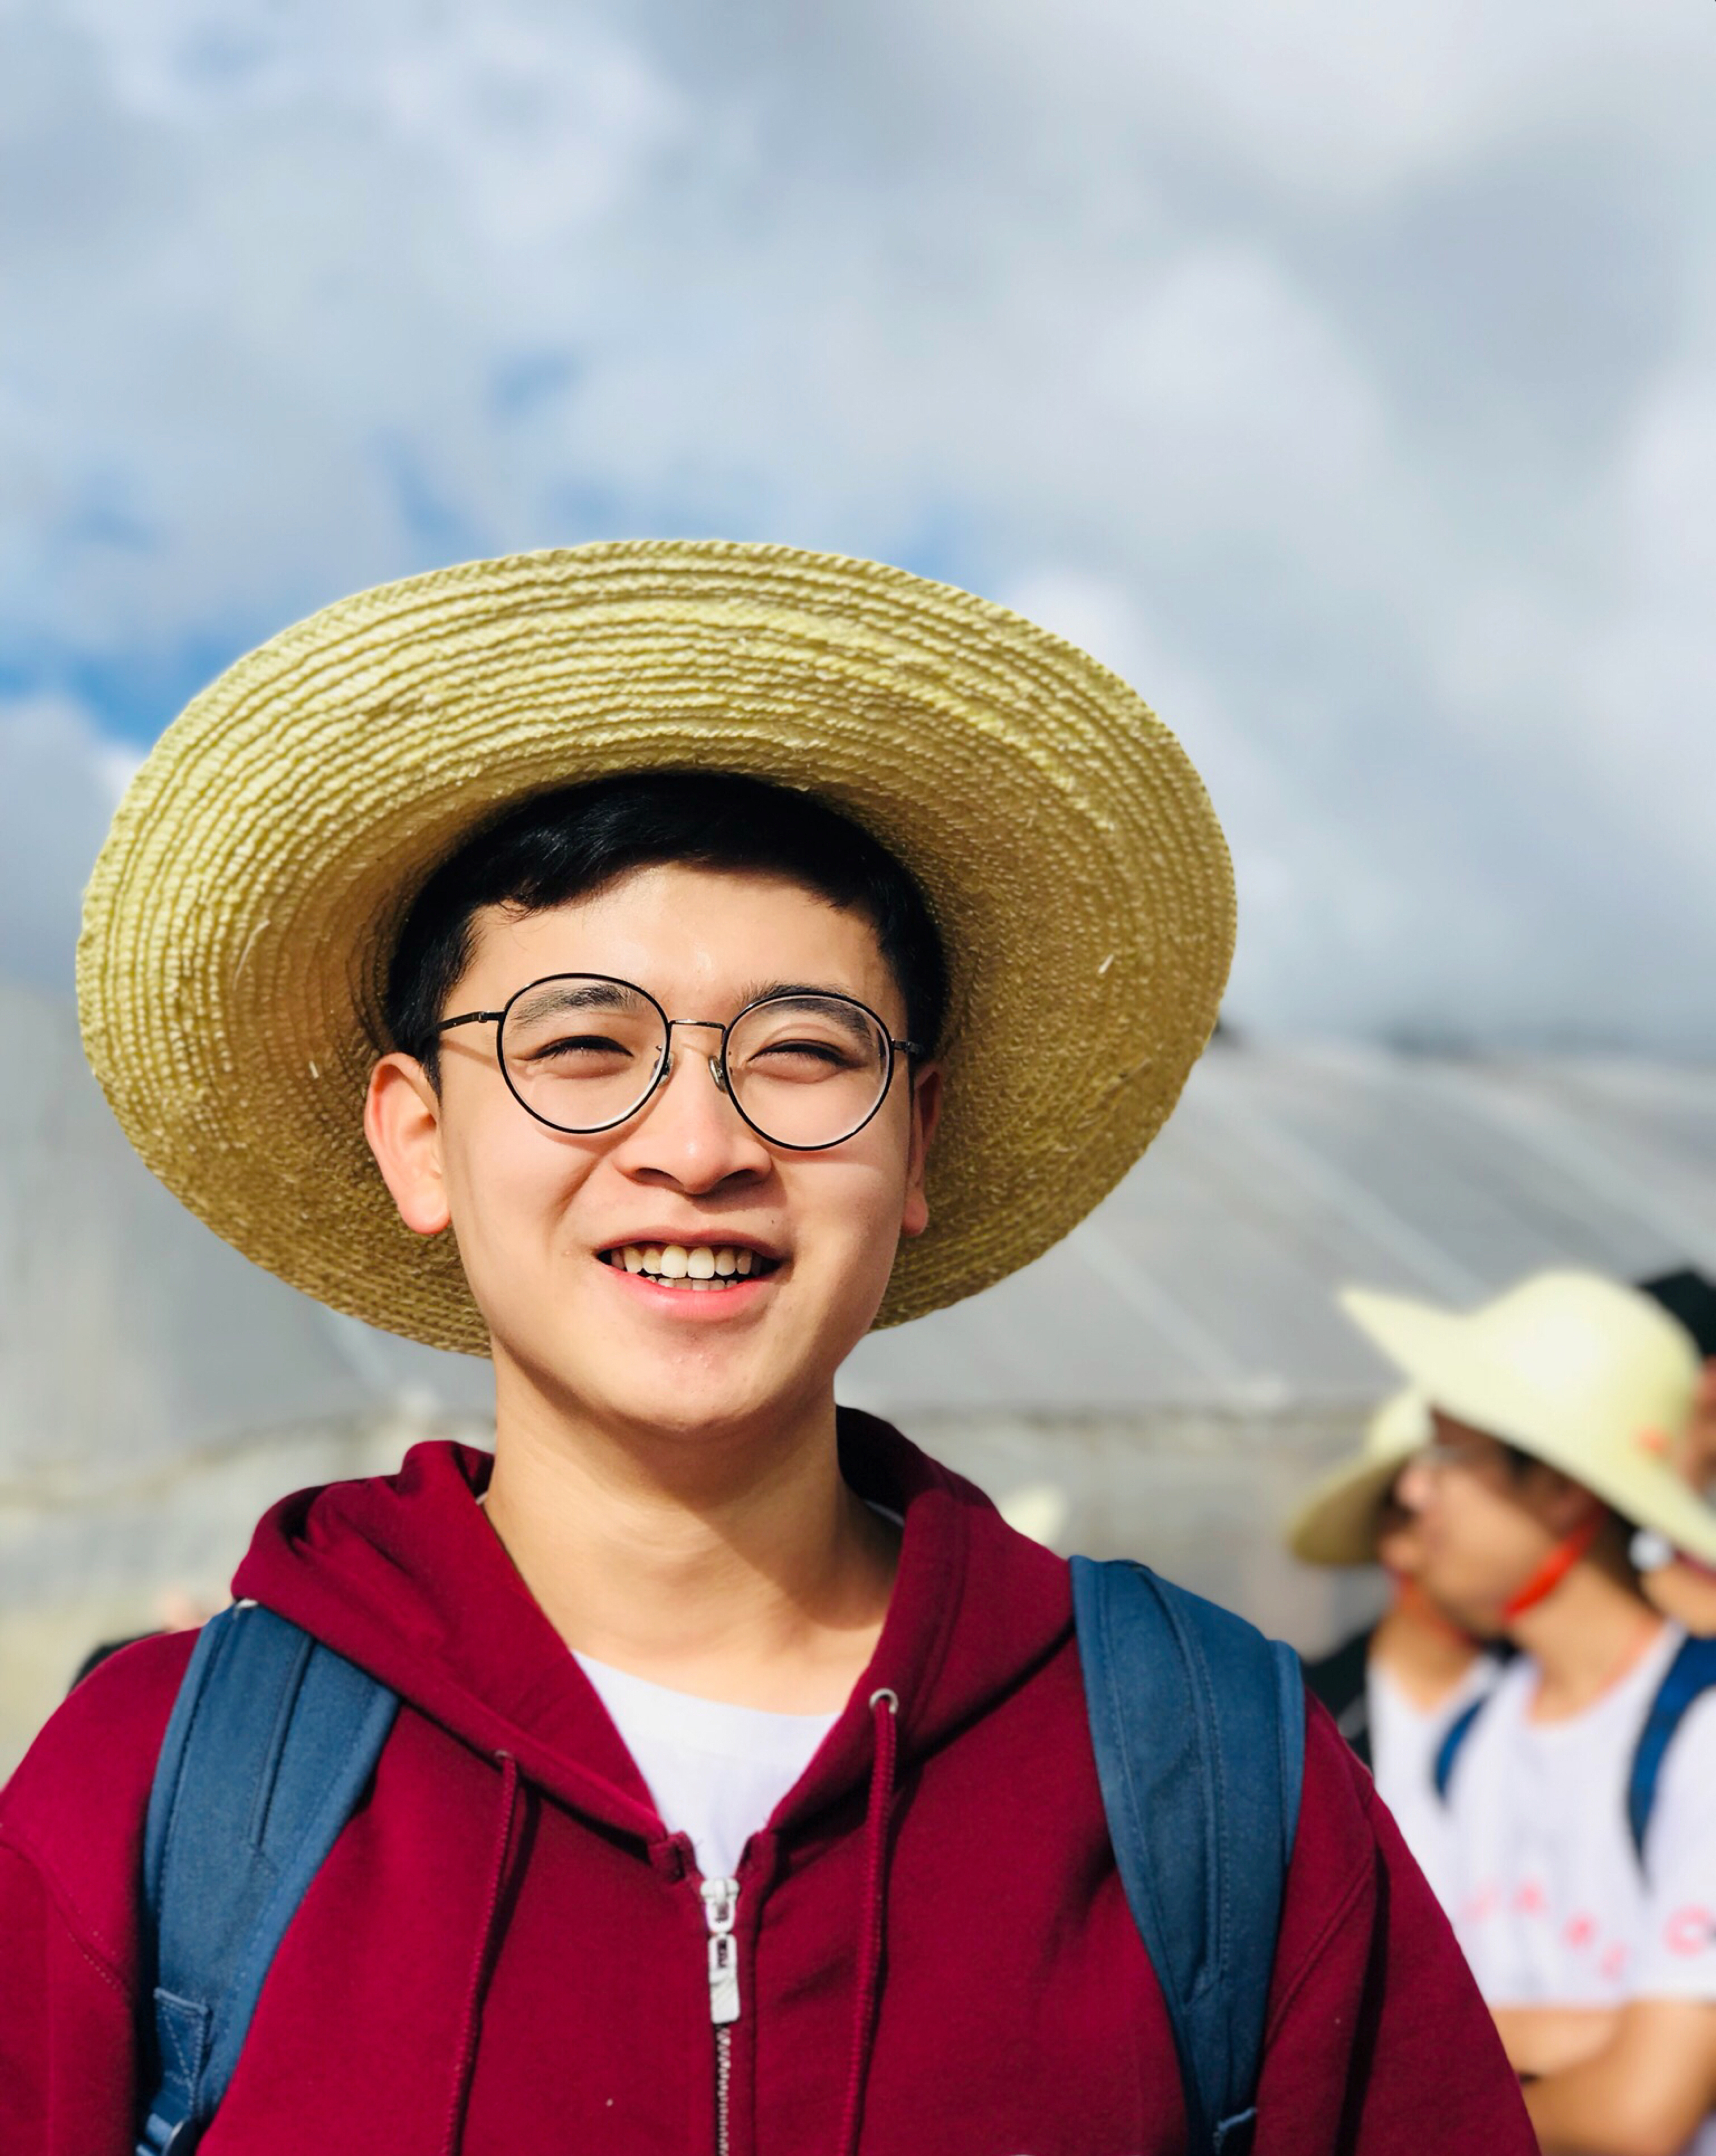
\includegraphics[width=0.45\textwidth]{images/1a.jpg}
    }
    \subfigure[背景替换效果图]{
        \includegraphics[width=0.45\textwidth]{images/1b}
    }
    \subfigure[影视人物原图]{
        \includegraphics[width=0.45\textwidth]{images/2a.jpg}
    }
    \subfigure[背景替换效果图]{
        \includegraphics[width=0.45\textwidth]{images/2b.jpg}
    }
    \subfigure[动物原图]{
        \includegraphics[width=0.45\textwidth]{images/3a.jpg}
    }
    \subfigure[背景替换效果图]{
        \includegraphics[width=0.45\textwidth]{images/3b.jpg}
    }

    \caption{选择人物图片进行预处理}
\end{figure}
\end{itemize}

\section{第二阶段计划}
\subsection{完成算法}
\par{\qquad 当前完成的算法部分可以实现基本功能,但是边缘等细节处理以及重组后的图片效果还不是很好,以及部分像素点的处理会有一定的误差,所以下一阶段的首要任务是对于现有算法进行性能完善。同时当前算法是python语言编写的,还需要改写成c语言,包括考虑到应用中图片的实际格式对部分代码进行一定的修改,为下一步开发提供便利。}
\subsection{学习Android开发}
\par{\qquad 因为最终要实现的是将算法应用到软件中,因此在算法部分完成后,下一步对于Android开发也需要进行一定的学习。同时,目前我们只是对于Linphone的源码框架有了一些了解,在开发之前还需要更为细致地对其分析,对各部分功能有更好的把握。这是在下个阶段中难度最大的部分,也是项目完成中最为关键的基础。}
\subsection{软件开发}
\par{\qquad 计划在第二阶段汇报之前,已经开始着手对于Linphone进行二次开发和功能拓展,这也是本项目的最后一部分。}

\end{document}
